% Tretji del predavanja: od dobre prosojnice nasveta 6 do konca, v temi
% Metropolis in razmerju 16 : 9. Na začetku vključi prva dva dela. O razdelitvi
% na tri dokumente glej stevilke.tex, o zgradbi predavanja pa berlin-4-3.tex.
% Ta del nima ukazov \section, ker bi Metropolis zanje sam vstavil prosojnice z
% naslovi razdelkov.
\documentclass[aspectratio=169]{beamer}
\usepackage{../pomozno/prosojnice}
\usepackage{pdfpages}

\newcommand{\ukaz}[1]{\texttt{\textbackslash#1}}
% Pomanjšana prosojnica iz teme.pdf: prvi argument je stran, drugi ime teme.
\newcommand{\tema}[2]{%
  \begin{minipage}[t]{0.32\textwidth}
    \centering
    \fbox{\includegraphics[page=#1, width=0.95\textwidth]{teme}}\\[-0.5ex]
    {\tiny #2}
  \end{minipage}%
}

% Prosojnica s kodo, ki vsebuje \end{frame}. Okolje frame z možnostjo fragile
% se konča pri prvi vrstici \end{frame}, tudi če je ta v kodi, zato take
% prosojnice zapišemo v okolju okvir, ki se konča pri \end{okvir}.
\newenvironment{okvir}{\begin{frame}[fragile,environment=okvir]}{\end{frame}}

% Pomanjšana prosojnica iz metropolis.pdf; argument je stran.
\newcommand{\demo}[1]{%
  \fbox{\includegraphics[page=#1, width=0.28\textwidth]{metropolis}}%
}

\begin{document}

% Prva dva dela obdržita svojo velikost strani.
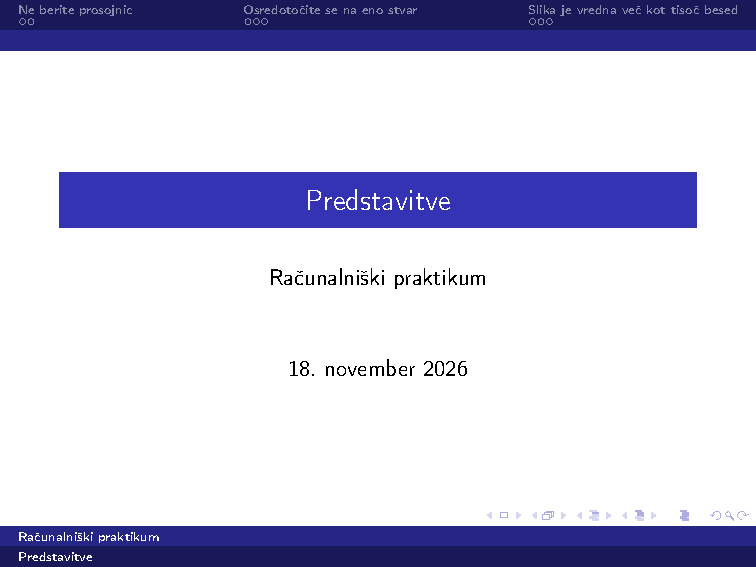
\includepdf[pages=-, fitpaper]{berlin-4-3.pdf}
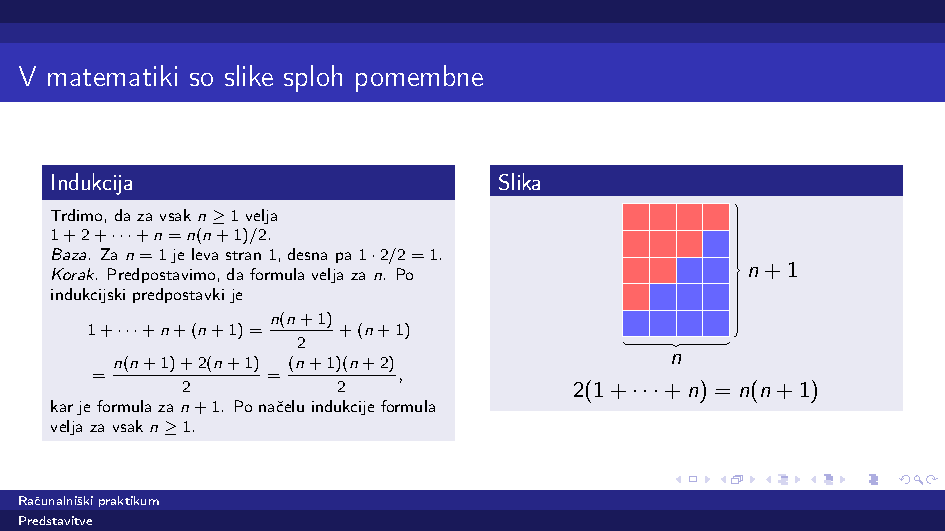
\includepdf[pages=-, fitpaper]{berlin-16-9.pdf}
\input{berlin-16-9.stevec}

% Šest strani iz predstavitve, ki jo TeX Live priloži temi Metropolis. Izvožene
% so iz zbornice, predavanja/08-predstavitve/izvoz.sh.
\begin{frame}[fragile]{Raje uporabite temo z boljšimi privzetimi nastavitvami}
  \begin{minted}{latex}
\usetheme{metropolis}
  \end{minted}
  \centering
  \demo{1}\hfill\demo{2}\hfill\demo{3}

  \smallskip
  \demo{4}\hfill\demo{5}\hfill\demo{6}

  {\tiny Primeri iz predstavitve teme Metropolis (Matthias Vogelgesang, CC BY-SA 4.0).}
\end{frame}

% Ista prosojnica v šestih Beamerjevih temah. Slike so izvožene iz zbornice,
% predavanja/08-predstavitve/izvoz.sh.
\begin{okvir}{Ne skačite po prosojnicah}
  \centering
  \tema{1}{Madrid}\hfill\tema{2}{Warsaw}\hfill\tema{3}{AnnArbor}

  \tema{4}{Antibes}\hfill\tema{5}{PaloAlto}\hfill\tema{6}{Darmstadt}
\pause

  \begin{minted}[fontsize=\footnotesize]{latex}
\begin{frame}[label=oznaka] ... \end{frame}
\againframe{oznaka}
  \end{minted}
\end{okvir}

\begin{frame}[fragile]{Vrstice naj ne bodo predolge}
  \onslide<1>{Bralec težko bere predolge vrstice, daljše od 80 znakov. Če res želite napisati daljše besedilo, ga vsaj razdelite v stolpce.}
  \begin{columns}[T]
    \begin{column}{0.4\textwidth}
      \onslide<2>{Bralec težko bere predolge vrstice, daljše od 80 znakov. Če res želite napisati daljše besedilo, ga vsaj razdelite v stolpce.}
    \end{column}
    \begin{column}{0.5\textwidth}
      \begin{minted}[fontsize=\footnotesize]{latex}
\begin{columns}
  \begin{column}{0.4\textwidth}
    Bralec težko bere ...
  \end{column}
  \begin{column}{0.5\textwidth}
    ...
  \end{column}
\end{columns}
      \end{minted}
    \end{column}
  \end{columns}
\end{frame}

% Fotografija: Forest Service Northern Region, Meadow Creek Campfire (2013),
% javna last, https://commons.wikimedia.org/wiki/File:Meadow_Creek_Campfire_(9194201298).jpg
% Fotografija v razmerju 3 : 2 zapolni širino prosojnice. Porežemo jo le
% zgoraj, kjer je nebo, da ogenj ostane cel.
{
  \setbeamertemplate{background}{%
    \vbox to \paperheight{\vss\hbox{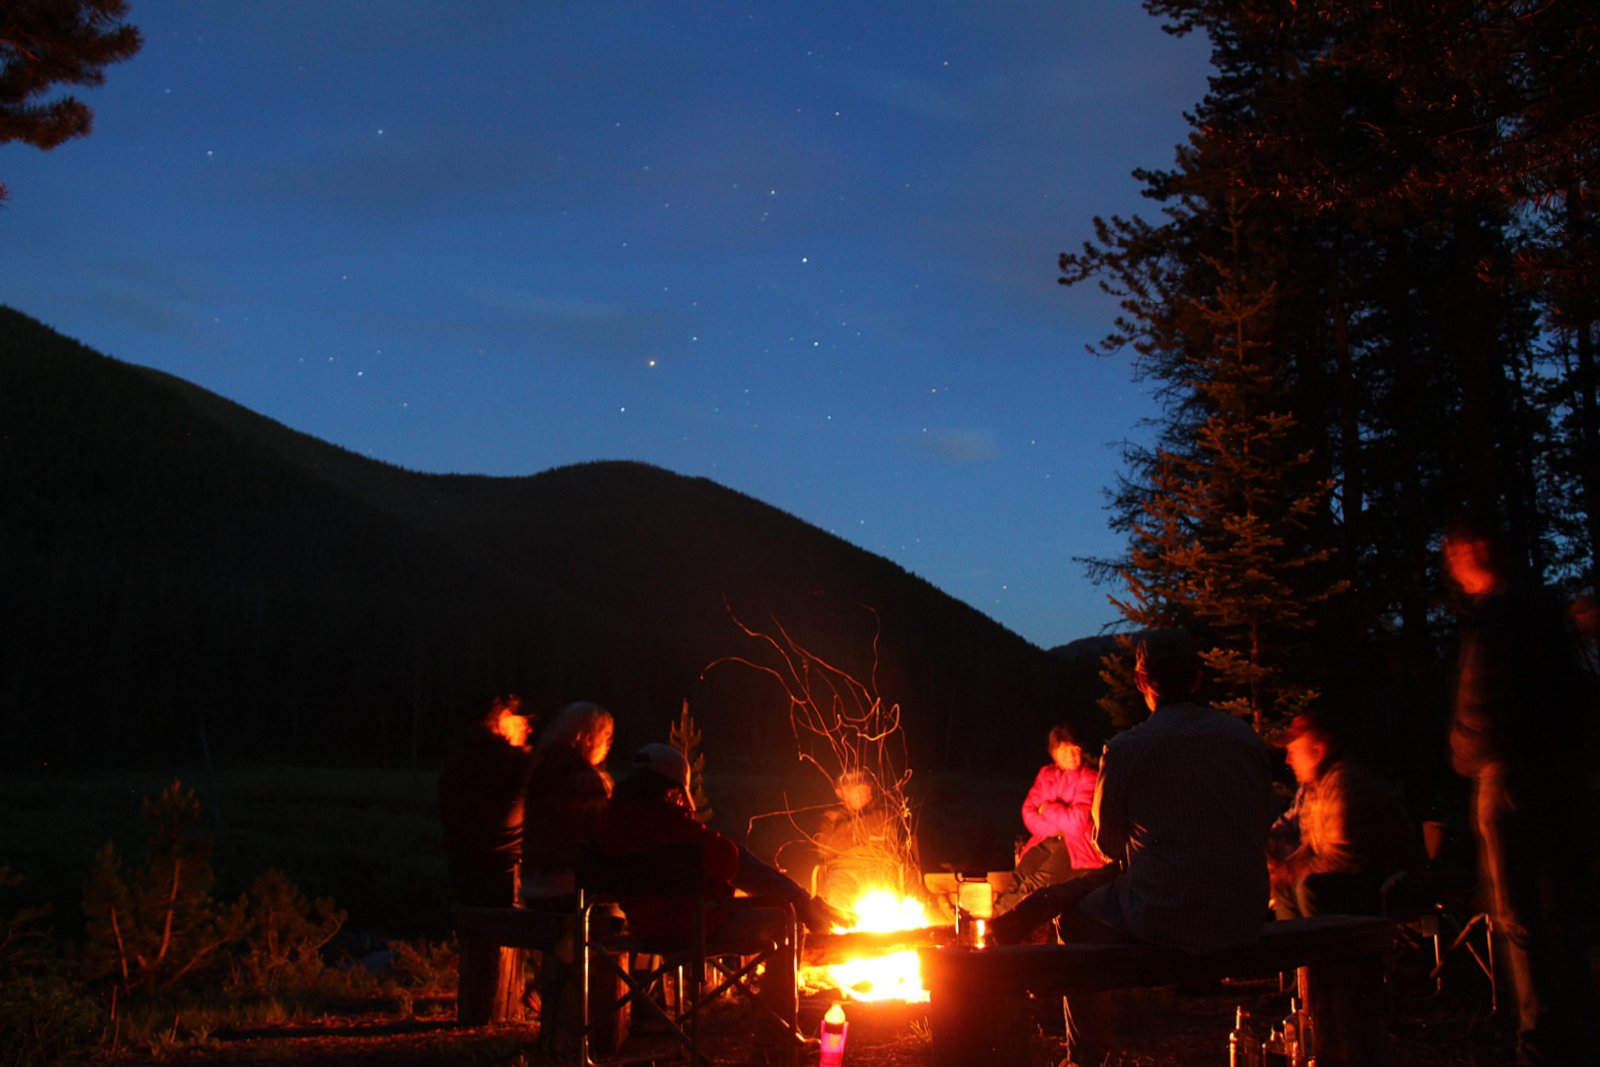
\includegraphics[width=\paperwidth]{taborni-ogenj}}}%
  }
  \begin{frame}
  \end{frame}
}

\end{document}
